\documentclass[12pt, a4paper]{article}
\usepackage[utf8]{inputenc}
\usepackage{graphicx}
\usepackage[margin=0.5in]{geometry}

\title{
\includegraphics{logo.png}\\Whork: Software Requirement Specification}
\author{Elio Magliari, Michele Tosi and Stefano Belli}
\date{}

\interfootnotelinepenalty=10000

\begin{document}
\maketitle
\section{Introduction}
\subsection{Aim of the document}
The following document contains a general description of the developed project, attached to it, you can find
design diagrams and storyboards.
\subsection{Overview of the defined system}
Whork is an easy to use job-seeking platform. It allows job seekers to find and candidate for a job based on their interests, with direct interaction such as
chatting with recruiter who posted this offer, immediate candidacy, on-sight workplace location map and only some other really useful details: no waste of time with useless infos.
Provides user-friendly job offer posting feature for company recruiters. Lets company admin able to manage recruiters by providing
a simple control panel in their own private profile. This system also ensures that company whose signing up is a valid one and we also mark
valid and secure offers with a "Verified by Whork" signature. Also, as previously said, a reliable chatting platform is built-in Whork, which can be used from recruiters to chat with
anyone who tries to reach them (by seeing their "inbox" in own private profile), job seekers will try to reach recruiter easily, just by pressing a button. Company admins and recruiters
can see general stats about their recruiting operations, like number of clicks on offers, number of posted offers, how many offers some recruiter posted, candidate employment status, and so on...
\subsection{Operational settings}
This system runs on whatever operating sytstem/architecture supports a java runtime environment.\\
 Fully works on Java JRE 11 or higher.
\subsection{Related systems}
These are our competitors:
\begin{itemize}
	\item Cercolavoro (https://www.cercolavoro.com/)
	\begin{itemize}
		\item Whork pro: realtime chat with recruiter
		\item Whork con: job cannot be filtered by particular area, province or comune
	\end{itemize}
	\item Indeed (https://it.indeed.com/)
	\begin{itemize}
		\item Whork pro: realtime chat with recruiter
		\item Whork con: job cannot be filtered by particular area, province or comune
	\end{itemize}
\end{itemize}

\section{User stories}
Various user stories are collected here:
\begin{itemize}
	\item As an user, I want to search for jobs using search filters,
		so that I can only see the offers that interest me.
	\item As a company, I want to manage my interview calendar, 
		so that I can organize my time and interviews. (???)
	\item As an user, I want to be notified by email when a company 
		offers a new job, so that I can schedule an interview. (???)
	\item As a job seeker, I want to have a map indicating where the workplace is,
		so that I can immediately see how far I am from it.
	\item As a job seeker, I want to directly chat with company's recruiter,
		so that I can have more specific infos about the job.
	\item As a company admin, I want to directly manage my recruiters,
		so that I can easily let them publish their field of expertise's offers
	\item As a company, I want to read the freelancers‘ CV, 
		so that I can choose the most experienced. (???)
	\item As a company, I want to post new job offers with candidature 
		requirements, so that I can easily find better employees. (???)
	\item As a candidate, I want to sort job offers based on salary, 
		so that I can choose the most profitable.  (???)
\end{itemize}

\section{Functional requirements}
The following are functional requirements for the project:
\begin{itemize}
	\item The system shall provide the ability to display a calendar for time management. (???)
	\item The system shall notify you by email of new offers from a favorite company. (???)
	\item The system shall provide the possibility to search based on the user's interest using advanced search filters.
	\item The system shall send a confirmation email after a job seeker successfully candidates for a job offer
	\item The system shall force every user to login before chatting with a recruiter
	\item The system shall check if a company's VAT code is valid or not, if it is not, then reject signup request.
	\item The system shall provide all users with an upload curriculum feature in their profile.
	\item The system shall provide all companies with a job posting function with attributes that let the job seeker 
	able to filter offers based on his/her interests
	\item The system shall sort job offers based on salary (descending order) on the search page. (???)
\end{itemize}

\newpage
\section{Use cases}
The following is a UML use case diagram for Whork:

\begin{center}
	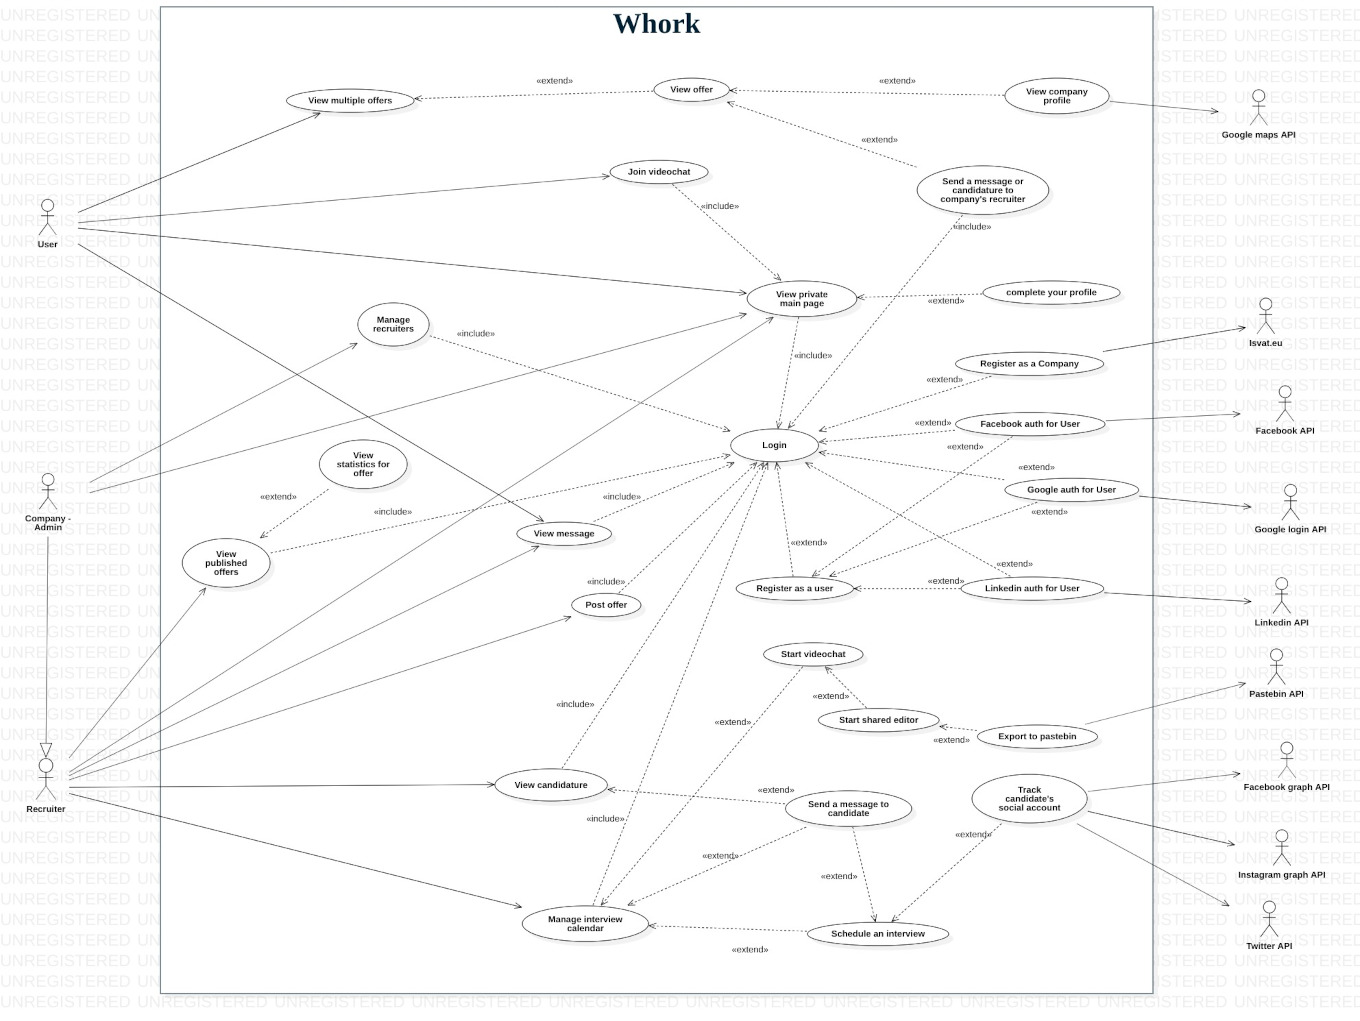
\includegraphics[scale=1.7]{diagrams/project/usecase/usecase_scaled.jpg}
\end{center}

\section{Dictionary}

\begin{itemize}
	\item \textit{Job Seeker} : some person looking for a job 
	\item \textit{Company Recruiter} : a recruiter for a company, who can post offer
	\item \textit{Company Admin} : an admin which is able to add more recruiters (an admin can also be a recruiter itself)
	\item \textit{Offer} : A job offer for whork which is composed of multiple attributes such as title, salary, work shift, workplace location, etc...
\end{itemize}

\end{document}
